\documentclass{article}

\usepackage[utf8x]{inputenc}
\usepackage[english,russian]{babel}
\usepackage{cmap}
\usepackage{commath}
\usepackage{amsmath}
\usepackage{amsfonts}
\usepackage{mathtools}
\usepackage{amssymb}
\usepackage{parskip}
\usepackage{titling}
\usepackage{color}
\usepackage{hyperref}
\usepackage{cancel}
\usepackage{enumerate}
\usepackage{multicol}
\usepackage{graphicx}
\usepackage[font=small,labelfont=bf]{caption}
\usepackage[a4paper, left=2.5cm, right=1.5cm, top=2.5cm, bottom=2.5cm]{geometry}

\graphicspath{ {./images/} }
\setlength{\droptitle}{-3cm}
\hypersetup{ colorlinks=true, linktoc=all, linkcolor=blue }
\pagenumbering{arabic}

\begin{document}
    \subsection{Понятие равномерной непрерывности}

    Рассмотрим функцию \(f(x)\) непрерывную в некотором "промежутке"(\(\infty\), конечные, открытые, закрытые).

    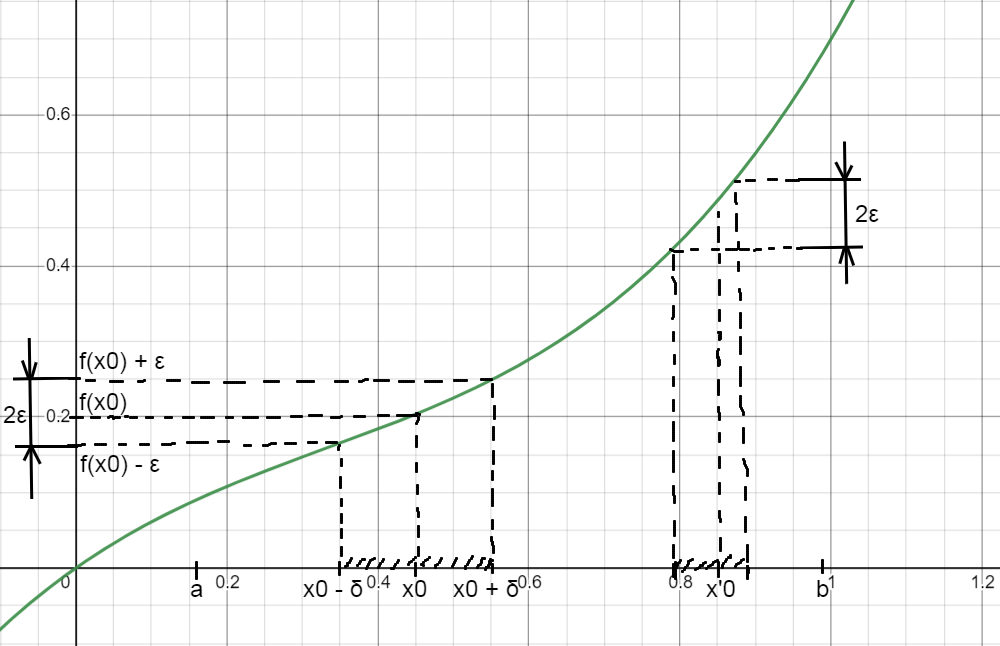
\includegraphics[width=\linewidth]{11_1_5_1.png}

    \(lim_{x \rightarrow x_0} f(x) = f(x_0)\)

    \(\forall \varepsilon > 0\ \exists\ \delta(\varepsilon):\ \forall x:\ \abs{x-x_0} < \delta\ \abs{f(x)-f(x_0)}<\varepsilon\).

    Если \(x \in X\), то \(\delta\ ||\ \varepsilon;\ x_0\).

    \textbf{Определение.} Будем говорить, что функция \(y = f(x)\) является равномерно непрерывной на некотором "промежутке" \(X\), если \(\forall \varepsilon > 0\ \exists\ \delta(\varepsilon)^{\textrm{не зависит от } x',x''}:\ \forall x',x'' \in X:\ \abs{x'-x''} < \delta\ \abs{f(x')-f(x'')} < \varepsilon\).
    
    \subsubsection{Теорема Кантора о равномерной непрерывности}

    \textbf{Теорема.} Функция \( f(x) \) непрерывная на \( [a; b] \) является и равномерно непрерывной на нём.
    
    \(\uparrow\) От противного.
    
    \begin{enumerate}
        \item \(\exists\ \varepsilon > 0:\ \forall \delta\ \exists\ x', x'':\ \abs{x' - x''} < \delta\), при этом \(\abs{f(x')-f(x'')} \geq \varepsilon\).
        \item Рассмотрим \(\delta_n \rightarrow 0\), для каждого из \(\delta_n \exists\ x_n', x_n'', \abs{x_n' - x_n''} < \delta_n\) и \(f(x_n') - f(x_n'') \geq \varepsilon(\star)\).
        \item Смотрим на \(x_n' \in [a; b]\), т.е. \(x_n'\) ограничена \(\Rightarrow\ \exists\) сходящаяся подпоследовательность \(x_{nk}':\ x_{nk}' \xrightarrow[k \rightarrow \infty]{} x_0 \in [a; b]\).
        \item Т.к. \( \abs{x_n' - x_n''} < \delta_n \)
        
        \( \Rightarrow lim_{n \to \infty}(x_n' - x_n'') = 0 \)

        \( \Rightarrow lim_{n \to \infty}(x_{nk}' - x_{nk}'') = 0\)

        \( \Rightarrow lim_{n \to \infty}(x_{nk}'') = lim_{n \to \infty}(x_{nk}') = x_0\)
        \item Функция \(f(x)\) непрерывна на \([a; b]\)
        
        \( lim_{k \to \infty}(f(x_{nk}')) = f(x_0) = lim_{k \to \infty}(f(x_{nk}'')) \)
        \item Тогда \( lim_{k \to \infty}(f(x_{nk}') - f(x_{nk}'')) = 0 \), но это противоречит (\(\star\))
        
        \( \abs{f(x_n') - f(x_n'')} \geq \varepsilon \)

        \( \abs{f(x_{nk}') - f(x_{nk}'')}_{\to 0} \geq \varepsilon \downarrow \)
    \end{enumerate}

    \textbf{Пример.}

    \begin{enumerate}
        \item \( y = \frac{1}{x} \) на \( (0; 1] \)

        (\( [\mu_{\textrm{фиксированное}}; 1] \) --- здесь равномерно непрерывна)
    
        Не являясь равномерно непрерывной \( \in (0; 1]\ \exists\ \varepsilon > 0:\ \forall\ \delta\ \exists\ x', x'':\ \abs{x' - x''} < \delta, \abs{f(x') - f(x'')} \geq \varepsilon \).
        
        Возьмём:
    
        \( x_n' = \frac{1}{n} = f(x) \)\\
        \( x_n'' = \frac{1}{2n} \)\\
        \( \abs{x_n' - x_n''} = \frac{1}{2n} < \delta \)\\
        \( \abs{f(x_n') - f(x_n'')} = \abs{n - 2n} = n \geq 1 \)\\
        \( \exists\ \varepsilon = 1:\ \forall\ \delta\ \exists\ x_n', x_n'':\ \abs{x_n' - x_n''} < \delta \), то \( \abs{f(x_n') - f(x_n'')} \geq 1\)
        
        \item \( y = x^2 \) на \( (0; 1) \)
        
        \( \abs{x_1^2 - x_2^2} = \abs{x_1 - x_2}\abs{x_1 + x_2} < 2\delta < \delta \)
    \end{enumerate}
    
    \section{Степенные функции}

    \subsection{Степенная функция с натуральным показателем}

    \textbf{Определение.} \(y = x^n;\ n \in \mathbb{N}\).
    
    \begin{enumerate}
        \item Область определения: \( x \in \mathbb{R}\).
        \item Непрерывна на всей области определения, как произведение произведение непрерывных.
        \item Возрастает при \(x \geq 0\).
        
        \(\uparrow\) Пусть \(x_1 > x_2 > 0\)(при \(x_2=0\) очевидно)

        \( f(x_1) - f(x_2) = x_1^n - x_2^n = (x_1 - x_2)(x_1^{n - 1} + x_2^{n - 2}x_2 + x_1^{n - 3}x_2^2 + ... + x_2^{n - 1}) \) 

        Первая скобка \( > 0 \), а вторая есть сумма положительных \( \Rightarrow f(x_1) > f(x_2) \Rightarrow \nearrow\) \(\downarrow\)
        
        Также в силу монотонности: \( 0 < x < 1 \Rightarrow 0 < x^n < 1 \), а также \(x > 1 \Rightarrow x^n > 1\)

        \item Чётность.
        
        \( n = 2k \), то \( y = x^n \) --- чётная \( \Rightarrow \) график симметричен.
        
        \(n = 2k + 1;\ y = x^n\) --- нечётная \(\Rightarrow\) график асимметричен.
        
        \item \(x^n;\ x^m,\ m < n\)

        \begin{enumerate}
            \item Если \(0 < x < 1\)

            \(x^n = x^{n-m}x^m < 1 * x^m\)

            \item Если \(x > 1\)

            \(x^n = x^{n-m}x^m > x^m\)
        \end{enumerate}
    
        \item При \( x \geq 0 \Rightarrow y = x^n \in [0; +\infty) \).
        \item При \( x \geq 0 \Rightarrow y = x^n \) принимает все значения \( \in [0; +\infty) \).

        \(\forall A \in [0; +\infty)\) надо показать \(\exists\ x_0:\ x_0^n = A\)

        \(\uparrow\) Т.к. \(lim_{x \rightarrow +\infty} x^n = +\infty\), то \(\forall A\ \exists\ c:\ c^n > A\). Тогда на \([0; c]\) пользуемся следствием 1 из т. Больцано, ч.т.д. \(\downarrow\)
        
    \end{enumerate}

    Из п. 7 и п. 3 получаем, что \( y = x^n \) взаимнооднозначное отображение "на" или \( y = x^n \) --- обратимая функция.

    \( y = x^n \Rightarrow\ \exists\ x = \sqrt[n]{y} \) или \( y = \sqrt[n]{x} \),
    
\end{document}
